\documentclass{oci}
\usepackage[utf8]{inputenc}
\usepackage{lipsum}

\title{Sistemas interestelares}

\begin{document}
\begin{problemDescription}
\begin{center}
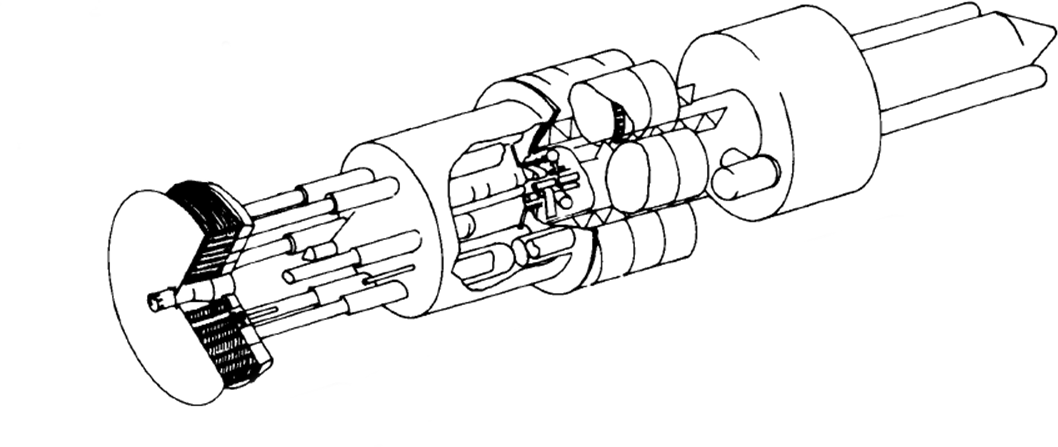
\includegraphics[scale=0.3]{interestellar.png}
\end{center}
La Oficina de Comunicaciones Interestelares (OCI) es una organización formada por distinguidos científicos de todo el mundo y encargada del estudio de comunicaciones a gran distancia.

La división de señales de alta potencia de la OCI ha descubierto recientemente un método para enviar señales con un alcance de cientos de años luz.
Para probarlo, se iniciará un programa de emisión de estas ondas de largo alcance.
Sin embargo, el programa es muy costoso, y en esta primera fase el presupuesto solo alcanza para emitir señales a 5 sistemas interestelares dentro de la Vía Láctea.
Para apoyar el trabajo de la división de Búsqueda de Vida Extraterrestre (BVET), el directorio de la OCI ha decidido que el destino de estas señales sea determinado por los científicos de la BVET.

La principal actividad de la BVET consiste en el análisis de ondas de radio provenientes de sistemas interestelares dentro de nuestra galaxia.
Esporádicamente, aparecen pulsaciones que podrían indicar la presencia de vida extraterrestre.
Sus equipos monitorean estas pulsaciones registrando para cada evento el sistema de donde provino.

La BVET decidió emitir las señales a los cinco sistemas que hayan registrado más eventos con pulsaciones, pues esto indicaría una mayor probabilidad de existencia de vida extraterrestre.
Sin embargo, sus equipos han registrado muchos eventos y están teniendo problemas para determinar cu\'ales son los 5 sistemas con más eventos.
Tú, que has sido recientemente contratado por la OCI, debes ayudar a los científicos de la BVET a tomar la decisión.

\end{problemDescription}

\begin{inputDescription}
La entrada consiste en varias líneas.
La primera línea contiene dos enteros $N$ y $S$ separados por un espacio.
$N$ corresponde a la cantidad de eventos que han sido registrados por los equipos de la BVET, y
$S$ corresponde a la cantidad de sistemas monitoreados.
Cada sistema es representado con un entero entre 1 y $S$.

Las siguientes $N$ líneas corresponden a cada uno de los eventos con pulsaciones.
Cada línea contiene un único entero $i$ ($1 \le i \le S$) correspondiente al sistema en el cual se detectó el evento.
Se garantiza que al menos habrán cinco sistemas para los cuales existen eventos.
\end{inputDescription}

\begin{outputDescription}
  Tu respuesta debe consistir en una única línea con cinco enteros separados por espacios.
  Estos deben corresponder a los cinco sistemas que registraron más eventos.
  Puedes imprimir estos enteros en cualquier orden.
  Si existe más de una solución puedes reportar cualquiera. (Mira la explicación luego de los casos de ejemplo.)
\end{outputDescription}

\begin{scoreDescription}
  \score{5} Se probarán varios casos donde $N=S=5$.
  \score{10} Se probarán varios casos donde $N=5$, $S=6$.
  \score{20} Se probarán varios casos donde $5 \le N \le 100$ y $5 \le S \le 100$.
  \score{30} Se probarán varios casos donde $100 < N \le 10^5$ y $100 < S \le 10^5$.
  \score{35} Se probarán varios casos donde $100 < N \le 10^5$ y $10^5 < S \le 10^9$.
\end{scoreDescription}

\begin{sampleDescription}
  \sampleIO{sample0}
  \sampleIO{sample1}
  \sampleIO{sample}
\end{sampleDescription}

Nota que dado que el orden de los valores en la respuesta no importa, en el primer caso de ejemplo otra 
posible respuesta v\'alida puede ser
\begin{center}
\texttt{5 4 3 2 1}
\end{center}
Por su parte, en el segundo caso de ejemplo otra posible respuesta v\'alida puede ser
\begin{center}
\texttt{1 6 3 5 4}
\end{center}

Si analizas el tercer caso de ejemplo, en los sistemas \texttt{6} y \texttt{7} se detectaron
3 pulsaciones, mientras que en los sistemas \texttt{1}, \texttt{2}, \texttt{4} y \texttt{5} 
se detectaron exactamente 2 pulsaciones, y en los demás sistemas no se detectaron pulsaciones. 
Por esto, las respuestas 
\begin{center}
\texttt{6 7 1 4 5}
\end{center}
y
\begin{center}
\texttt{6 7 2 4 5}
\end{center}
también serían válidas. 

Recuerda que independiente de la cantidad de respuestas válidas que existan tu programa
solo debe generar una de ellas.
\end{document}
